\documentclass[aspectratio=43,11pt]{beamer}

\usetheme{default}
\usecolortheme{default}
\definecolor{aggiemaroon}{RGB}{80,0,0}
\setbeamercolor{structure}{fg=aggiemaroon}
\setbeamertemplate{navigation symbols}{}
\setbeamertemplate{footline}[frame number]
\setbeamertemplate{itemize items}[circle]
\setbeamertemplate{enumerate items}[default]
\setbeamersize{text margin left=0.55cm,text margin right=0.55cm}

\usepackage[utf8]{inputenc}
\usepackage[T1]{fontenc}
\usepackage{lmodern}
\usepackage{amsmath,amssymb}
\usepackage{booktabs}
\usepackage{graphicx}
\usepackage{xcolor}
\usepackage{listings}
\usepackage{tikz}
\usetikzlibrary{arrows.meta,positioning}

\definecolor{codebg}{RGB}{247,247,247}
\definecolor{darkblue}{RGB}{20,64,120}
\definecolor{darkgreen}{RGB}{20,110,70}
\definecolor{darkred}{RGB}{160,50,50}

\lstdefinestyle{rcode}{
  language=R,
  basicstyle=\ttfamily\scriptsize,
  backgroundcolor=\color{codebg},
  frame=single,
  rulecolor=\color{gray!35},
  columns=fullflexible,
  keepspaces=true,
  showstringspaces=false,
  breaklines=true,
  breakatwhitespace=true,
  tabsize=2,
  commentstyle=\color{darkgreen},
  keywordstyle=\color{darkblue},
  stringstyle=\color{darkred},
  xleftmargin=0.4em,
  xrightmargin=0.4em
}
\lstdefinestyle{stancode}{
  language=C,
  basicstyle=\ttfamily\scriptsize,
  backgroundcolor=\color{codebg},
  frame=single,
  rulecolor=\color{gray!35},
  columns=fullflexible,
  keepspaces=true,
  showstringspaces=false,
  breaklines=true,
  breakatwhitespace=true,
  tabsize=2,
  commentstyle=\color{darkgreen},
  keywordstyle=\color{darkblue},
  stringstyle=\color{darkred},
  xleftmargin=0.4em,
  xrightmargin=0.4em
}
\lstset{style=rcode}

\newcommand{\smallnote}[1]{\vspace{0.25em}{\fontsize{8}{0}\selectfont\color{gray!65!black}#1\par}}
\newcommand{\source}{\smallnote{Based on Bayes Rules!, Chapter 6: Approximating the Posterior.}}
\newcommand{\tightitems}{\setlength\itemsep{0.25em}}

\title{Decision and Risk Analysis}
\subtitle{Lecture 7: \textbf{Approximating the Posterior}\\
{\it Grid Approximation, MCMC, and RStan}
}
\author{}
\date{
\color{aggiemaroon}{
DAEN 427 / ISEN 427 / ISEN 627 - Fall 2026\\
\textbf{Alexander Abuabara}
}
}
\titlegraphic{\vfill 
\includegraphics[height=1.2cm]{TAMU_logo.png}}

\begin{document}

% 1
\begin{frame}
  \titlepage
\end{frame}

% 2
\begin{frame}{Learning goals}
%By the end, students should be able to:
\begin{enumerate}\tightitems
  \item Explain why posterior approximation is needed.
  \item Implement grid approximation in R.
  \item Explain the basic idea of MCMC and RStan.
  \item Read basic MCMC diagnostics: trace plots, autocorrelation, effective sample size, and R-hat.
  \item Use posterior draws for practical risk decisions.
\end{enumerate}

\vspace{1em}
\begin{center}
simple exact model $\rightarrow$ grid approximation $\rightarrow$ \\ \qquad \qquad \qquad $\rightarrow$ MCMC $\rightarrow$ RStan $\rightarrow$ diagnostics $\rightarrow$ decisions
\end{center}
\end{frame}

% 3
\begin{frame}{Example}
A supplier says that most parts pass inspection.\\
We test 10 parts and 9 pass.

\vspace{0.25em}
\begin{columns}[T]
\column{0.48\textwidth}
\textbf{Unknown}
\[
\pi=P(\text{part passes})
\]

\textbf{Prior}
\[
\pi\sim\text{Beta}(2,2)
\]
This prior is centered near 0.5,\\but still uncertain.

\column{0.48\textwidth}
\textbf{Data model}
\[
Y\mid\pi\sim\text{Bin}(10,\pi),\qquad Y=9
\]

\textbf{Risk question}
\[
P(\pi<0.70\mid Y=9)?
\]
If this is high,\\inspect more or reject the supplier.
\end{columns}
\end{frame}

% 4
\begin{frame}{Bayesian update}
\[
\pi\mid Y=9\sim\text{Beta}(2+9,\;2+1)=\text{Beta}(11,3).
\]
\begin{center}
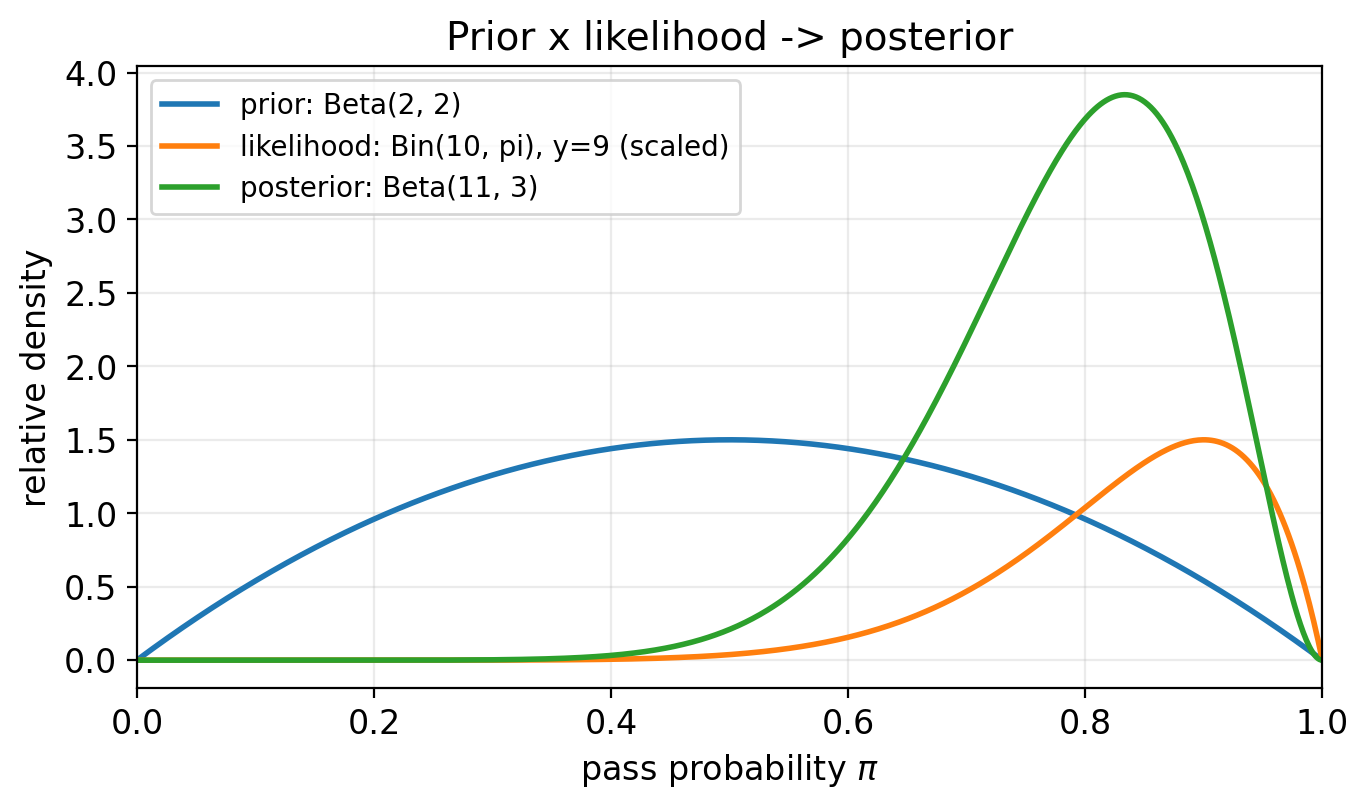
\includegraphics[width=0.86\linewidth]{lecture7_figures/beta_update.png}
\end{center}
\vspace{-0.6em}
\smallnote{Let us use a simple model because the exact posterior is known,\\and the approximation methods can be checked.}
\end{frame}

% 5
\begin{frame}{Why approximate at all?}
For simple models, we can sometimes write the posterior exactly:
\[
f(\theta\mid y)=\frac{f(\theta)L(\theta\mid y)}{f(y)}.
\]

For realistic models, $\theta$ may contain many parameters:
\[
\theta=(\theta_1,\theta_2,\ldots,\theta_k).
\]

Then the normalizing constant may require a hard integral:
\[
f(y)=\int\cdots\int f(\theta)L(\theta\mid y)d\theta.
\]

\begin{block}{}
Produce draws $\theta^{(1)},\theta^{(2)},\ldots,\theta^{(N)}$ that behave like posterior draws.
\end{block}
\end{frame}

% 6
\begin{frame}{Two approximation ideas}
\begin{columns}[T]
\column{0.48\textwidth}
\begin{block}{1. Grid approximation}
\begin{itemize}\tightitems
  \item Try many possible parameter values.
  \item Score each value by prior $\times$ likelihood.
  \item Normalize scores into probabilities.
  \item Sample from the discrete grid.
\end{itemize}
\end{block}

\column{0.48\textwidth}
\begin{block}{2. MCMC}
\begin{itemize}\tightitems
  \item Build a dependent sequence of values.
  \item Each next value depends on the current value.
  \item A good chain mimics the posterior.
  \item RStan handles the sampling algorithm.
\end{itemize}
\end{block}
\end{columns}

\vspace{0.3em}
\begin{center}
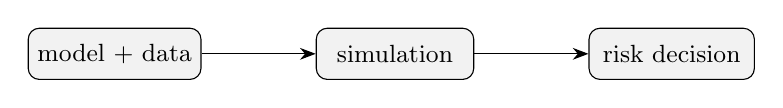
\begin{tikzpicture}[node distance=1.45cm,every node/.style={font=\small}]
\node[draw,rounded corners,fill=gray!10,minimum width=2.1cm,minimum height=0.65cm] (model) {model + data};
\node[draw,rounded corners,fill=gray!10,right=of model,minimum width=2.0cm,minimum height=0.65cm] (sim) {simulation};
\node[draw,rounded corners,fill=gray!10,right=of sim,minimum width=2.1cm,minimum height=0.65cm] (dec) {risk decision};
\draw[-{Stealth[length=2.0mm]}] (model) -- (sim);
\draw[-{Stealth[length=2.0mm]}] (sim) -- (dec);
\end{tikzpicture}
\end{center}
\end{frame}

% 7
\begin{frame}{Grid approximation algorithm}
\textbf{Goal:} approximate $f(\theta\mid y)$ using a finite set of possible values.

\begin{enumerate}\tightitems
  \item Define a grid of possible $\theta$ values.
  \item Evaluate the prior and likelihood at each grid value.
  \item Multiply and normalize:
  \[
  \text{posterior probability}=\frac{\text{prior}\times\text{likelihood}}{\sum \text{prior}\times\text{likelihood}}.
  \]
  \item Sample grid values using those posterior probabilities.
\end{enumerate}

\begin{block}{Intuition}
A grid is like viewing a curve through many vertical slices.\\
More slices give a clearer picture.
\end{block}
\end{frame}

% 8
\begin{frame}[fragile]{Grid approximation in R}
\begin{lstlisting}[style=rcode]
# Y | pi ~ Bin(10, pi), pi ~ Beta(2, 2), observed Y = 9
library(tidyverse)

# Step 1: choose grid points
grid_data <- data.frame(pi_grid = seq(0, 1, length = 101))

# Step 2: evaluate prior and likelihood on the grid
grid_data <- grid_data %>%
  mutate(prior = dbeta(pi_grid, 2, 2),
         likelihood = dbinom(9, size = 10, prob = pi_grid))

# Step 3: prior x likelihood, then normalize
grid_data <- grid_data %>%
  mutate(unnormalized = prior * likelihood,
         posterior = unnormalized / sum(unnormalized))
\end{lstlisting}
\smallnote{Key coding idea: each row is one possible value of $\pi$.\\
The posterior column is a probability distribution across rows.}
\end{frame}

% 9
\begin{frame}[fragile]{Grid approximation in R}
\begin{lstlisting}[style=rcode]
set.seed(84735)

# Step 4: sample grid values using posterior probabilities
post_sample <- sample_n(grid_data, size = 10000,
                        weight = posterior, replace = TRUE)

# Use the sample like posterior draws
post_sample %>%
  summarize(mean_pi = mean(pi_grid),
            q05 = quantile(pi_grid, 0.05),
            q95 = quantile(pi_grid, 0.95),
            risk_low_quality = mean(pi_grid < 0.70))
\end{lstlisting}
\begin{block}{}
After step 4, the posterior sample is the main object.\\
Summaries, intervals, and risk probabilities all come from it.
\end{block}
\end{frame}

% 10
\begin{frame}{Coarse grid (few values)}
\begin{center}
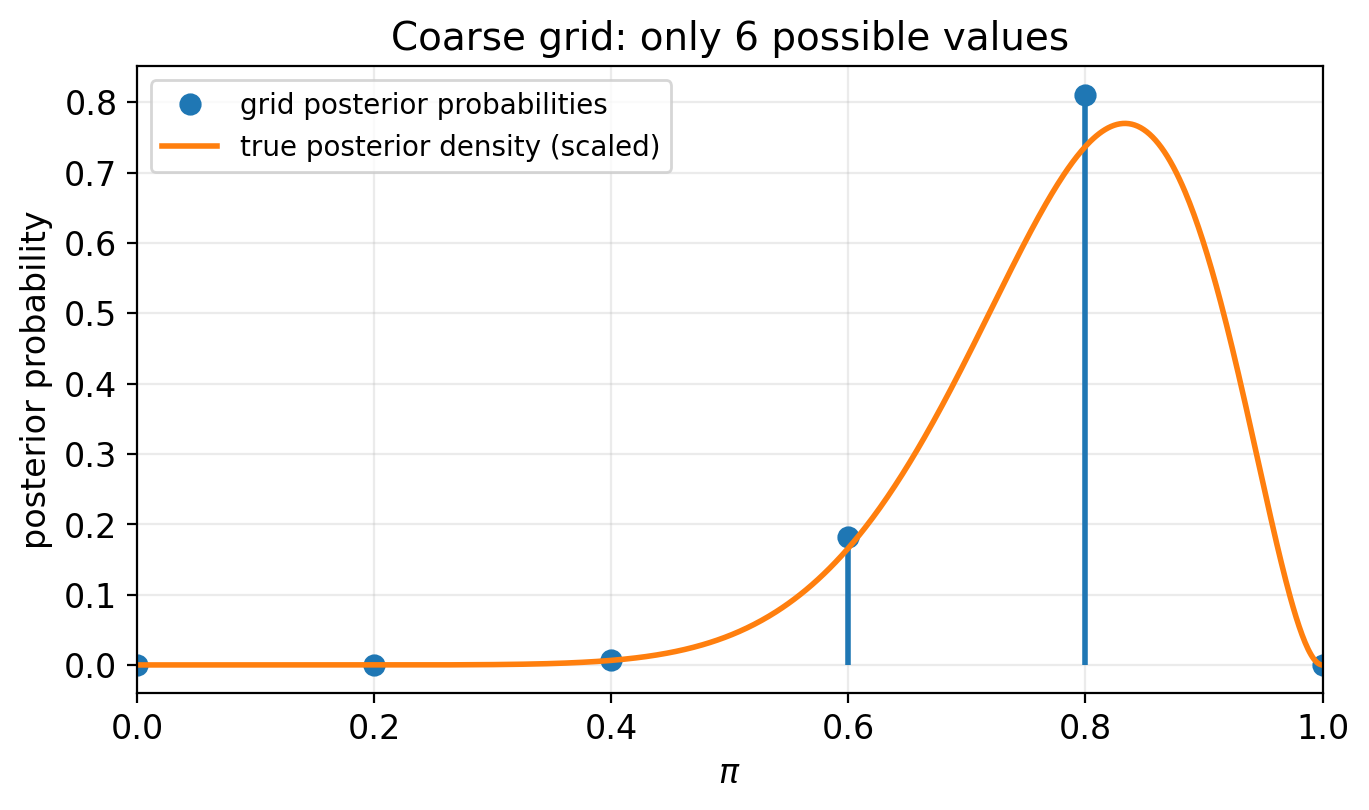
\includegraphics[width=0.7\linewidth]{lecture7_figures/coarse_grid.png}
\end{center}
\vspace{-0.5em}
With only 6 grid points, the posterior can only place mass at
\[
0,\;0.2,\;0.4,\;0.6,\;0.8,\;1.0.
\]
This is easy to understand, but too rigid for careful risk analysis.
\end{frame}

% 11
\begin{frame}{Finer grid (approximation improves)}
\begin{center}
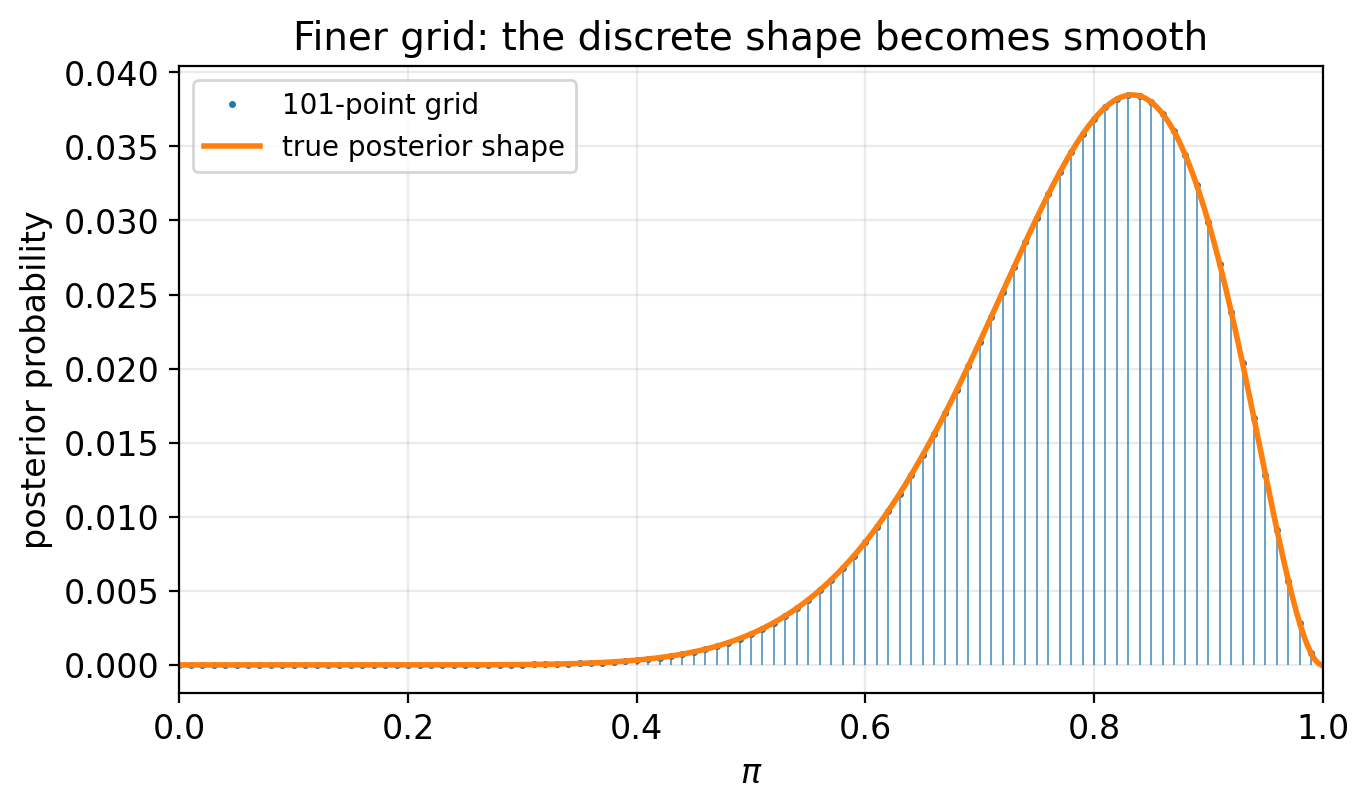
\includegraphics[width=0.7\linewidth]{lecture7_figures/fine_grid.png}
\end{center}
\vspace{-0.5em}
\begin{itemize}
\item Using 101 grid values makes the discrete approximation look much closer to the smooth posterior. (usually improves accuracy)
\item But also increase computation.
\end{itemize}
\end{frame}

% 12
\begin{frame}{Using posterior draws for a decision}
\begin{center}
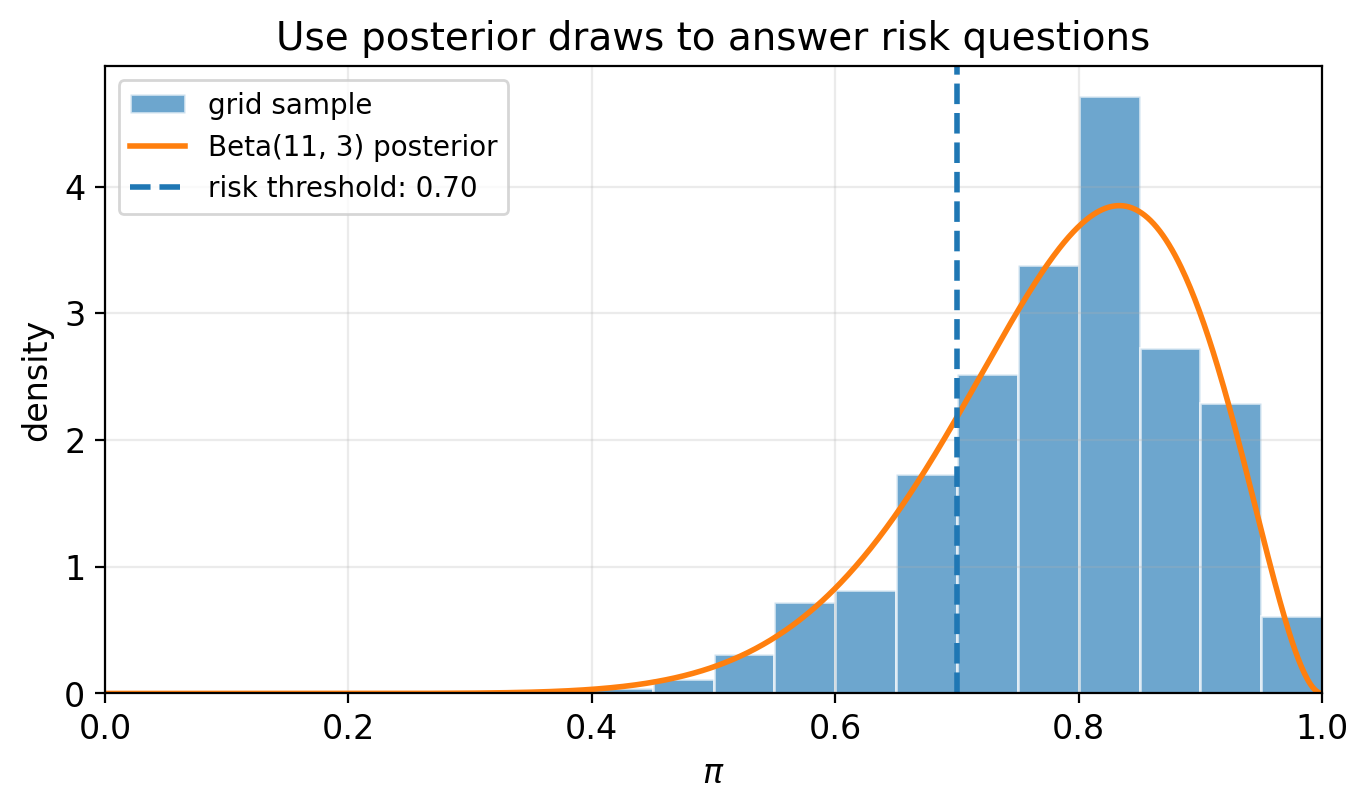
\includegraphics[width=0.7\linewidth]{lecture7_figures/risk_decision_beta.png}
\end{center}
\vspace{-0.5em}
For the supplier example:
\[
E(\pi\mid y)\approx0.786,\qquad P(\pi<0.70\mid y)\approx0.20.
\]
\textbf{Decision rule:} if $P(\pi<0.70\mid y)>0.10$,\\
collect more evidence or reject the supplier.
\end{frame}

% 13
\begin{frame}{Second example: events per hour}
Suppose an industrial engineer monitors events per hour:
\begin{itemize}\tightitems
  \item machine stoppages,
  \item helpdesk tickets,
  \item safety incidents,
  \item truck arrivals at a dock.
\end{itemize}

Let $\lambda$ be the event rate per hour:
\[
Y_i\mid\lambda\sim\text{Pois}(\lambda),\qquad \lambda\sim\text{Gamma}(3,1).
\]

We observe two one-hour counts:
\[
y=(2,8),\qquad \sum y_i=10.
\]

Exact conjugate result:
\[
\lambda\mid y\sim\text{Gamma}(3+10,\;1+2)=\text{Gamma}(13,3).
\]
\end{frame}

% 14
\begin{frame}[fragile]{Gamma-Poisson grid approximation in R}
\begin{lstlisting}[style=rcode]
# Event count example: Y = c(2, 8)
grid_data <- data.frame(lambda_grid = seq(0, 15, length = 501))

grid_data <- grid_data %>%
  mutate(prior = dgamma(lambda_grid, shape = 3, rate = 1),
         likelihood = dpois(2, lambda_grid) *
                      dpois(8, lambda_grid),
         unnormalized = prior * likelihood,
         posterior = unnormalized / sum(unnormalized))

set.seed(84735)
post_sample <- sample_n(grid_data, size = 10000,
                        weight = posterior, replace = TRUE)

post_sample %>%
  summarize(mean_lambda = mean(lambda_grid),
            risk_high_rate = mean(lambda_grid > 6))
\end{lstlisting}
\end{frame}

% 15
\begin{frame}{Gamma-Poisson}
\begin{center}
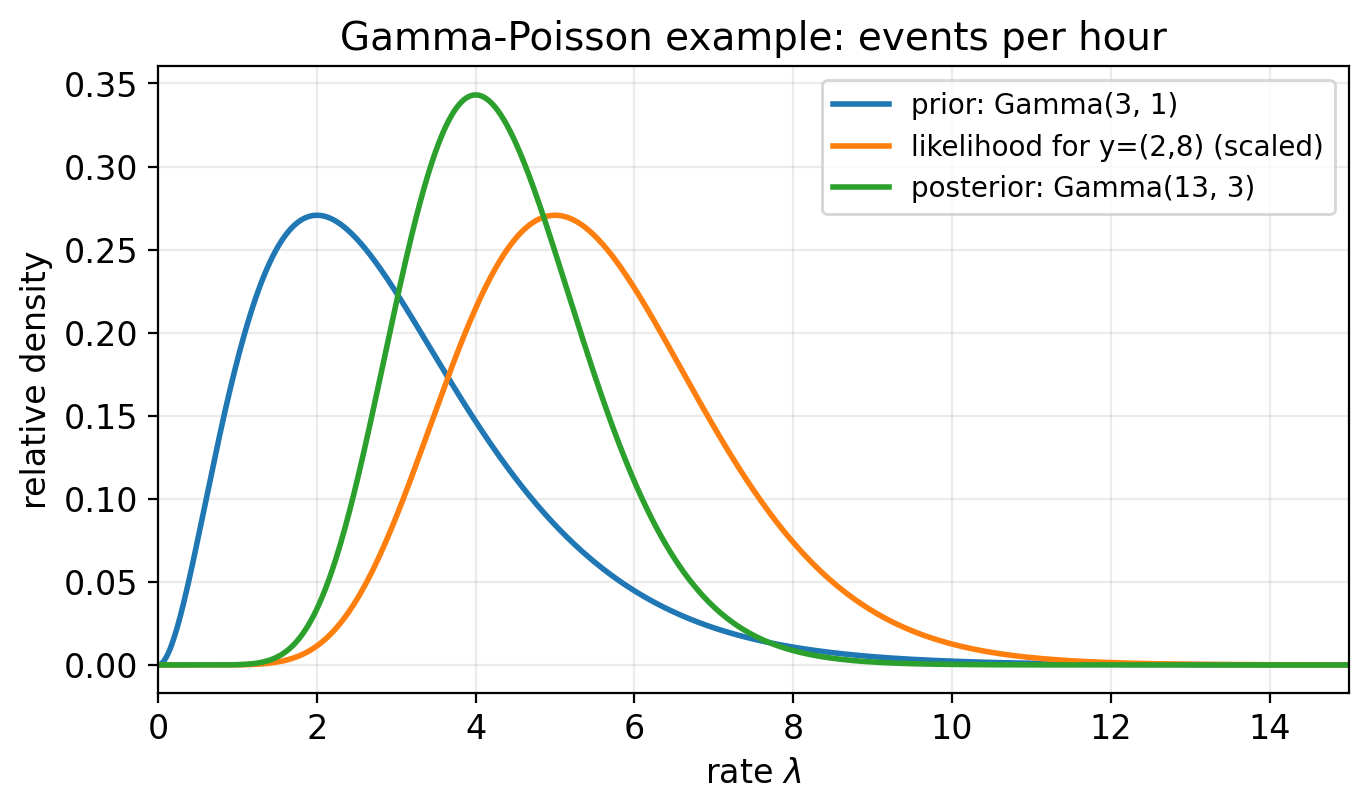
\includegraphics[width=0.7\linewidth]{lecture7_figures/gamma_poisson_update.png}
\end{center}
\vspace{-0.75em}
For $\lambda\mid y\sim\text{Gamma}(13,3)$:
\[
E(\lambda\mid y)\approx4.33,\qquad P(\lambda>6\mid y)\approx0.09.
\]
\textbf{Decision use:} decide whether capacity for more than 6 events/hour is necessary.
\end{frame}

% 16
\begin{frame}{Grid limitation (curse of dimensionality)}
\begin{center}
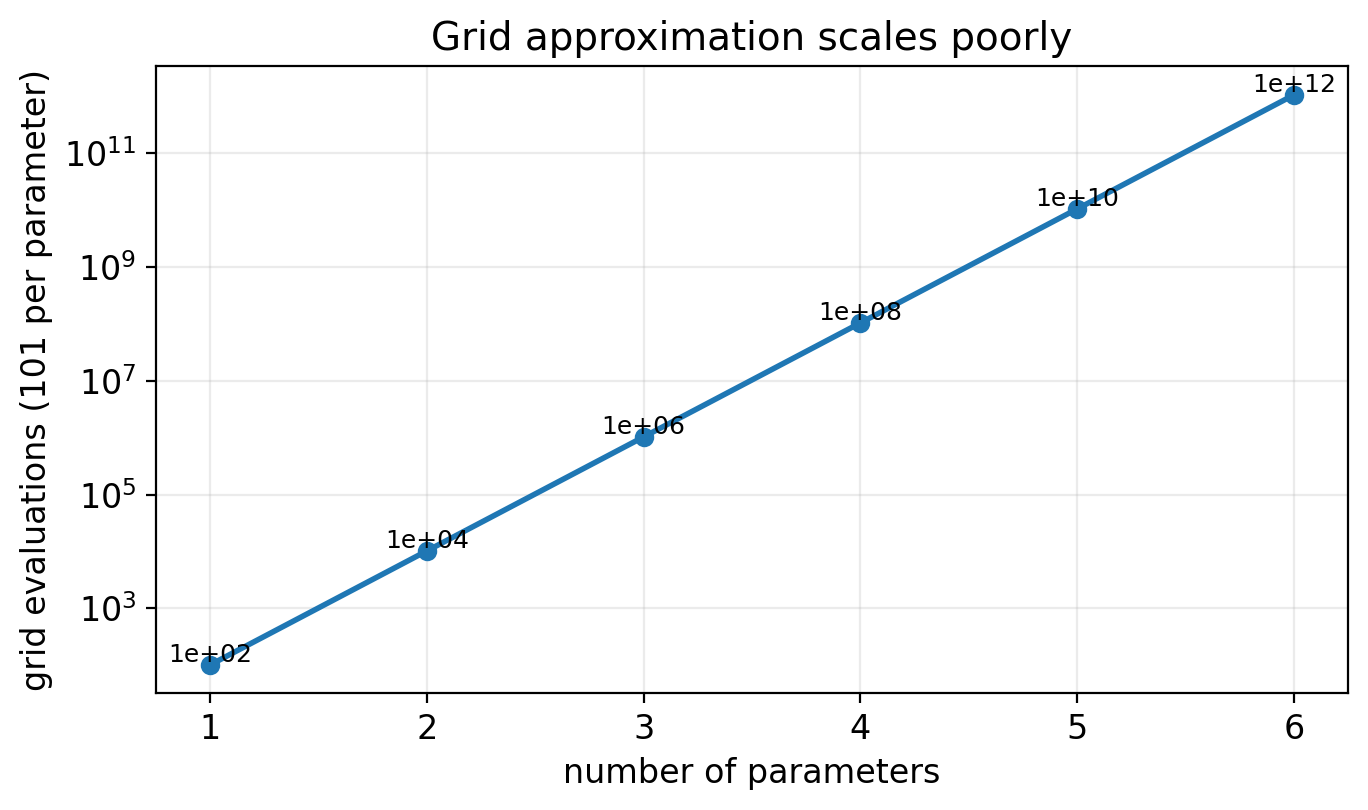
\includegraphics[width=0.70\linewidth]{lecture7_figures/curse_dimensionality.png}
\end{center}
\vspace{-0.5em}
If one parameter uses 101 grid values, then $k$ parameters require
$101^k$ grid evaluations. For 5 parameters, that is more than $10^{10}$.

\textbf{Main limitation:} 
Grid approximation is intuitive, but it does not scale well to many parameters.
\end{frame}

% 17
\begin{frame}{MCMC}
Grid approximation tries to evaluate many locations in advance.

MCMC instead makes a chain:
\[
\theta^{(1)}\rightarrow\theta^{(2)}\rightarrow\theta^{(3)}\rightarrow\cdots\rightarrow\theta^{(N)}.
\]

\begin{block}{Markov property}
The next draw depends on the current draw, not the full past:
\[
f(\theta^{(i+1)}\mid\theta^{(1)},\ldots,\theta^{(i)},y)
=f(\theta^{(i+1)}\mid\theta^{(i)},y).
\]
\end{block}

A good chain spends more time in plausible posterior regions and less time elsewhere.
\end{frame}

% 18
\begin{frame}{MCMC versus grid approximation}
\begin{table}
\centering
\scriptsize
\begin{tabular}{p{0.30\linewidth}p{0.29\linewidth}p{0.29\linewidth}}
\toprule
 & Grid approximation & MCMC \\
\midrule
Sample type & Independent draws from a discrete approximation & Dependent draws in a chain \\
Main strength & Very intuitive & Scales better to complex models \\
Main weakness & Curse of dimensionality & Requires diagnostics \\
Student image & Try every grid point & Walk around plausible regions \\
\bottomrule
\end{tabular}
\end{table}

\begin{block}{Caution:}
MCMC draws are not independent. We must check whether the chain mixed well enough to trust the approximation.
\end{block}
\end{frame}

% 19
\begin{frame}[fragile]{Stan declarations basic pattern}
A Stan declaration tells us three things:

\vspace{0.2cm}
\begin{center}
\texttt{type<constraints> name;}
\end{center}

Example:
\begin{lstlisting}[style=stancode]
real<lower=0, upper=1> theta;
\end{lstlisting}

\begin{center}
\scriptsize
\begin{tabular}{lll}
\toprule
\textbf{Part} & \textbf{Meaning} & \textbf{Example} \\
\midrule
\texttt{real} & decimal-valued number & 0.35, 2.1, -4.7 \\
\texttt{<lower=0, upper=1>} & allowed range & between 0 and 1 \\
\texttt{theta} & variable name & unknown probability \\
\bottomrule
\end{tabular}
\end{center}

Mathematically: \quad $0\leq\theta\leq1$.
\end{frame}

% 20
\begin{frame}[fragile]{Why use constraints?}
Constraints keep the model consistent with the meaning of the variable.

\begin{lstlisting}[style=stancode]
real<lower=0, upper=1> theta;
\end{lstlisting}

This is appropriate when $\theta$ is a probability:
\[
\theta=P(\text{component is defective}).
\]

A probability cannot be negative and cannot exceed 1.

\vspace{0.3cm}
Without the constraint:
\begin{lstlisting}[style=stancode]
real theta;
\end{lstlisting}
Stan would allow impossible values such as $-0.20$ or $1.40$.
\end{frame}

% 21
\begin{frame}[fragile]{Common Stan declarations}
\begin{center}
\scriptsize
\begin{tabular}{lll}
\toprule
\textbf{Stan declaration} & \textbf{Plain English} & \textbf{Typical use} \\
\midrule
\texttt{real mu;} & any decimal number & mean or intercept \\
\texttt{real<lower=0> sigma;} & nonnegative decimal & standard deviation \\
\texttt{real<lower=0,upper=1> p;} & probability & defect or success rate \\
\texttt{int<lower=1> N;} & integer at least 1 & sample size \\
\texttt{array[N] int<lower=0,upper=1> y;} & $N$ zeros/ones & binary outcomes \\
\texttt{vector[N] x;} & $N$ decimal values & predictor values \\
\bottomrule
\end{tabular}
\end{center}

\vspace{0.3cm}
Important: angle brackets \texttt{< >} do \textbf{not} mean ``less than'' here. They declare restrictions.

\vspace{0.2cm}
\begin{center}
\texttt{real<lower=0> sigma;} \quad means \quad $\sigma\geq0$.
\end{center}
\end{frame}

% 22
\begin{frame}[fragile]{RStan model structure: Beta-Binomial}
The Stan code is a direct translation of the model:
\[
Y\mid\pi\sim\text{Bin}(10,\pi),\qquad \pi\sim\text{Beta}(2,2).
\]

\begin{lstlisting}[style=rcode]
library(rstan)
library(bayesplot)

bb_model <- "
data {
  int<lower = 0, upper = 10> Y;
}
parameters {
  real<lower = 0, upper = 1> pi;
}
model {
  pi ~ beta(2, 2);
  Y ~ binomial(10, pi);
}
"
\end{lstlisting}
\smallnote{Data are supplied from R. Parameters are unknowns.\\
The model block contains prior and likelihood.}
\end{frame}

% 23
\begin{frame}[fragile]{RStan simulation command}
\begin{lstlisting}[style=rcode]
bb_sim <- stan(model_code = bb_model,
               data = list(Y = 9),
               chains = 4,
               iter = 5000 * 2,
               seed = 84735)
\end{lstlisting}

\begin{columns}[T]
\column{0.45\textwidth}
\textbf{Arguments}
\begin{itemize}\tightitems
  \item \texttt{model\_code}: Stan model string.
  \item \texttt{data}: observed data list.
  \item \texttt{chains}: parallel chains.
  \item \texttt{iter}: iterations per chain.
\end{itemize}

\column{0.48\textwidth}
\textbf{Warmup / burn-in}
\begin{itemize}\tightitems
  \item The first half is usually warmup.
  \item Warmup lets the algorithm adapt.
  \item The retained draws approximate the posterior.
\end{itemize}
\end{columns}
\end{frame}

% 24
\begin{frame}{Trace plots: first diagnostic}
\begin{center}
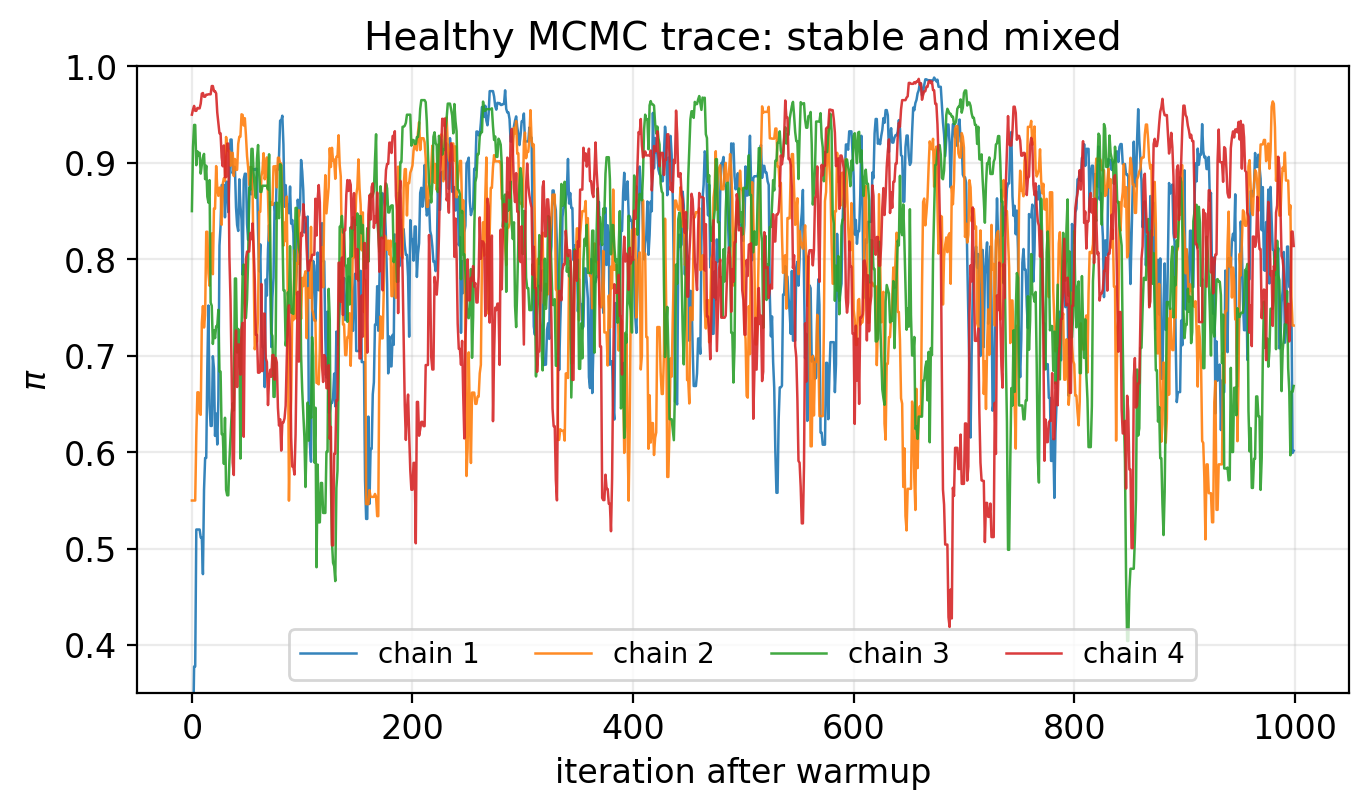
\includegraphics[width=0.7\linewidth]{lecture7_figures/mcmc_trace_good.png}
\end{center}
\vspace{-0.4em}
A healthy trace plot looks stable and noisy, with chains exploring the same range.

\textbf{Plain-language test:} does each chain wander around the same posterior region without a trend or long pause?
\end{frame}

% 25
\begin{frame}{Trace plots: warning signs}
\begin{center}
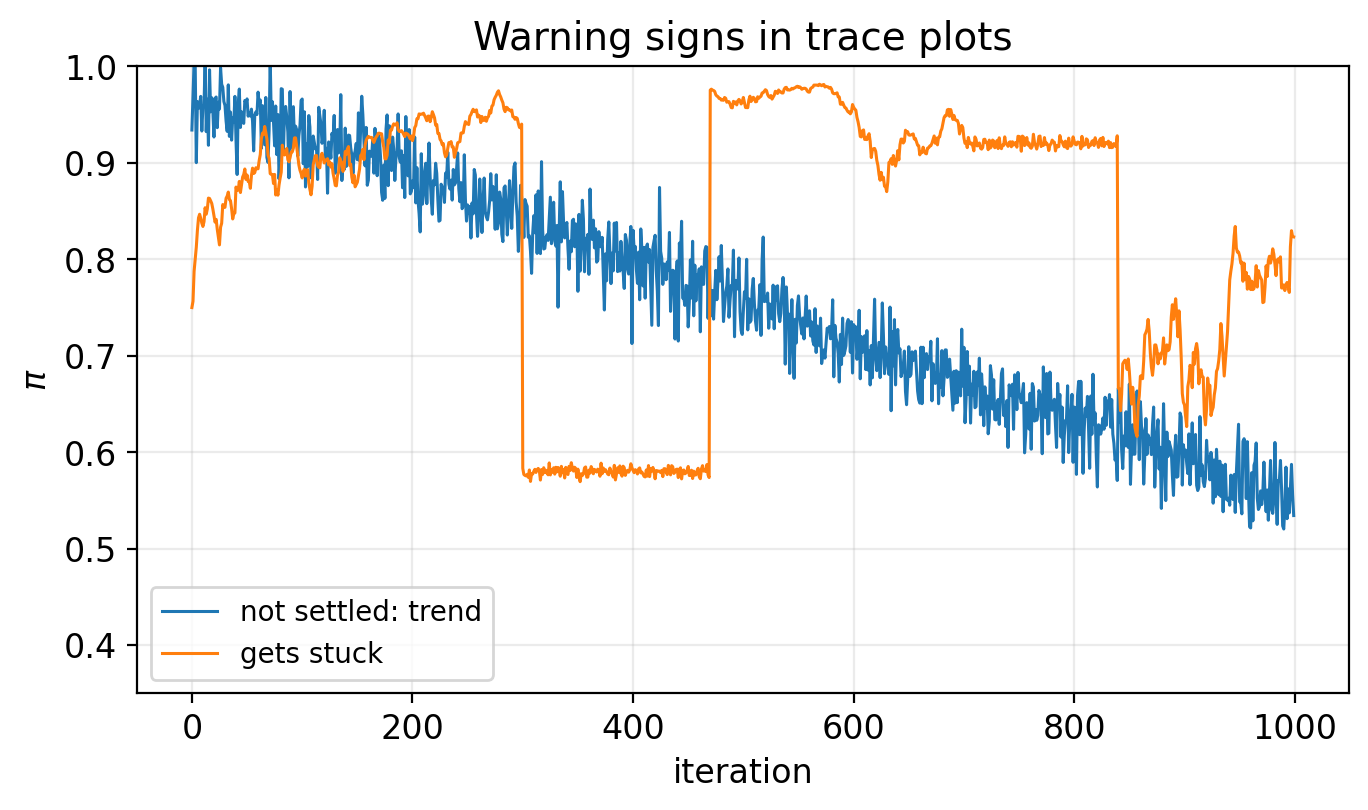
\includegraphics[width=0.7\linewidth]{lecture7_figures/mcmc_trace_bad.png}
\end{center}
\vspace{-0.5em}
\begin{itemize}\tightitems
  \item A trend suggests the chain has not settled.
  \item A flat section suggests the chain got stuck.
  \item Either problem can give misleading posterior summaries.
\end{itemize}
\end{frame}

% 26
\begin{frame}{Posterior distribution from MCMC draws}
\begin{center}
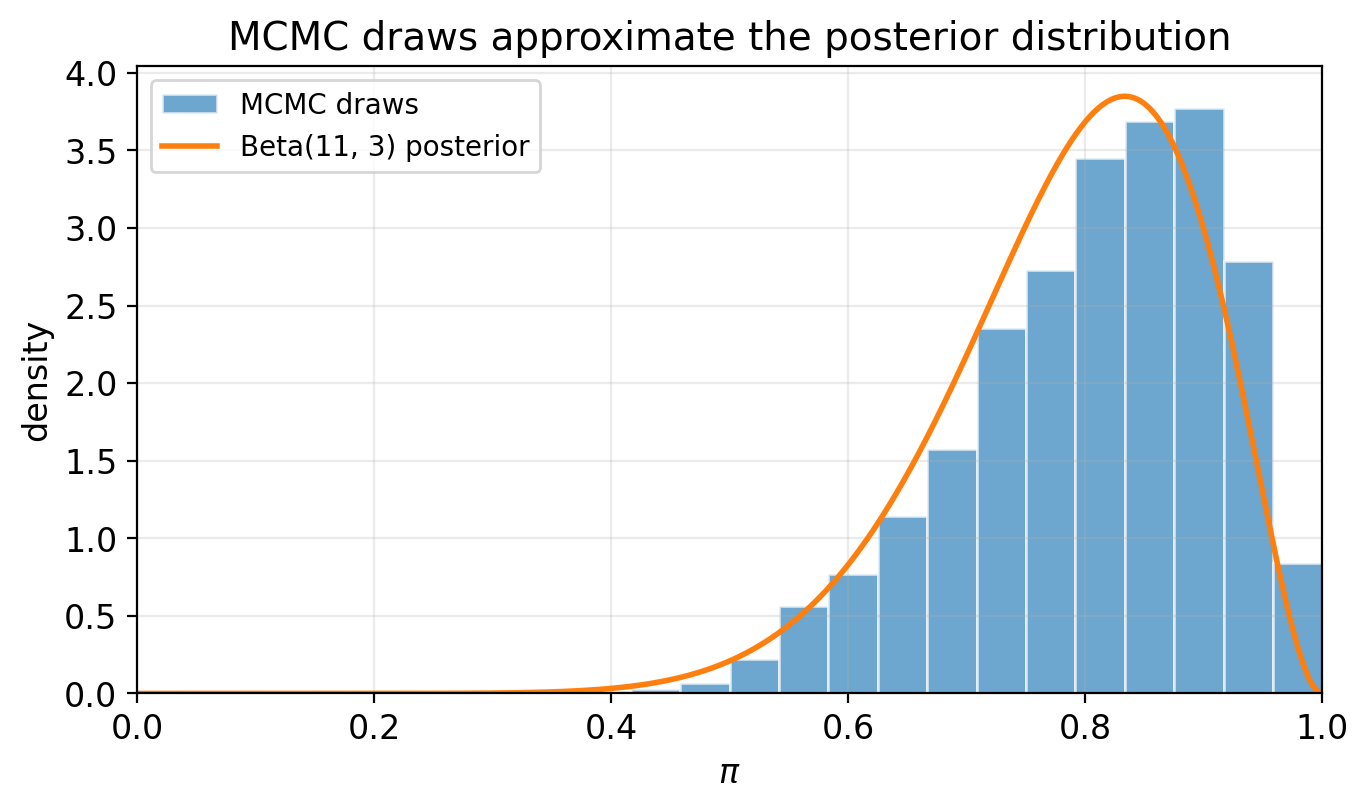
\includegraphics[width=0.7\linewidth]{lecture7_figures/mcmc_posterior_hist.png}
\end{center}
\vspace{-0.5em}
After diagnostics look acceptable, summarize retained draws just like a grid sample:
\[
\text{mean},\quad \text{credible interval},\quad P(\text{bad outcome}\mid y).
\]
\end{frame}

% 27
\begin{frame}[fragile]{Diagnostic code in R}
\begin{lstlisting}[style=rcode]
# Visual diagnostics
mcmc_trace(bb_sim, pars = "pi")
mcmc_dens_overlay(bb_sim, pars = "pi")
mcmc_acf(bb_sim, pars = "pi")

# Numerical diagnostics
neff_ratio(bb_sim, pars = "pi")
rhat(bb_sim, pars = "pi")
\end{lstlisting}

\begin{block}{How to read the diagnostics}
\begin{itemize}\tightitems
  \item Trace plot: stable, noisy, no trend, no long sticking.
  \item Density overlay: parallel chains should look similar.
  \item Autocorrelation: should drop quickly.
  \item Effective sample size ratio: larger is better.
  \item R-hat: should be close to 1; values above about 1.05 raise concern.
\end{itemize}
\end{block}
\end{frame}

% 28
\begin{frame}{Autocorrelation: fast versus slow mixing}
\begin{center}
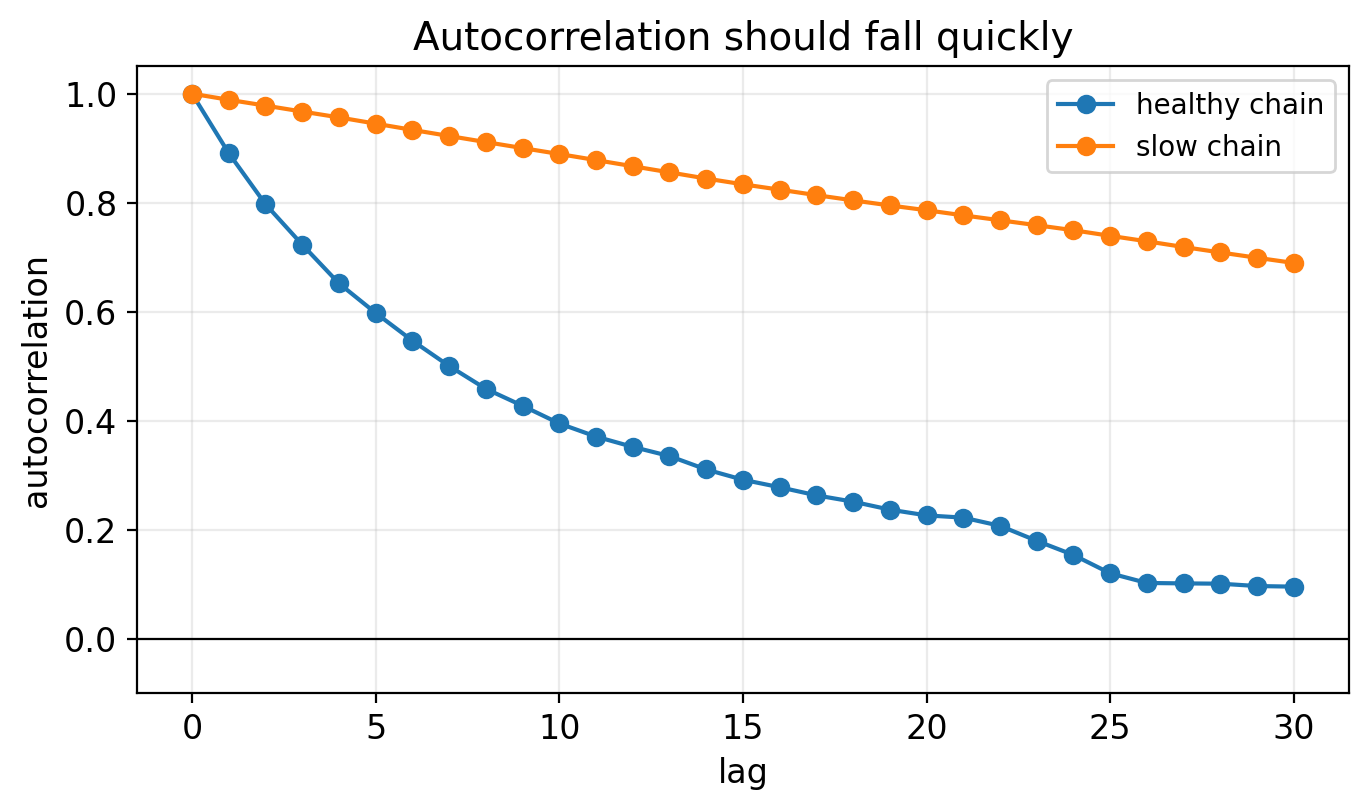
\includegraphics[width=0.7\linewidth]{lecture7_figures/autocorrelation.png}
\end{center}
\vspace{-0.5em}
Strong autocorrelation means nearby draws are very similar.

\begin{block}{Risk-analysis implication}
A chain with 20,000 highly correlated draws may contain much less information than 20,000 independent draws.
\end{block}
\end{frame}

% 29
\begin{frame}[fragile]{RStan model structure: Gamma-Poisson}
\begin{lstlisting}[style=rcode]
gp_model <- "
data {
  array[2] int<lower = 0> Y;
}
parameters {
  real<lower = 0> lambda;
}
model {
  lambda ~ gamma(3, 1);
  Y ~ poisson(lambda);
}
"

gp_sim <- stan(model_code = gp_model,
               data = list(Y = c(2, 8)),
               chains = 4,
               iter = 5000 * 2,
               seed = 84735)
\end{lstlisting}
\smallnote{Only the likelihood and prior change. The workflow stays the same.}
\end{frame}

% 30
\begin{frame}{Simple workflow}
\begin{enumerate}\tightitems
  \item Write the data model and prior.
  \item Use grid approximation if there are only one or two parameters.
  \item Use MCMC/RStan for more realistic models.
  \item Always inspect diagnostics before making decisions.
  \item Turn posterior draws into risk quantities:
  \[
  P(\text{failure rate too high}\mid y),\qquad
  E(\text{loss}\mid y).
  \]
\end{enumerate}

\begin{block}{}
The output is not just an estimate.\\
It is a distribution of plausible values for risk calculations.
\end{block}
\end{frame}

% 31
\begin{frame}[fragile]{Mini-exercise: change the supplier example}
Try a more skeptical prior and fewer successes:
\[
Y\mid\pi\sim\text{Bin}(10,\pi),\qquad \pi\sim\text{Beta}(3,8),\qquad Y=2.
\]

\begin{lstlisting}[style=rcode]
grid_data <- data.frame(pi_grid = seq(0, 1, length = 201)) %>%
  mutate(prior = dbeta(pi_grid, 3, 8),
         likelihood = dbinom(2, 10, pi_grid),
         unnormalized = prior * likelihood,
         posterior = unnormalized / sum(unnormalized))

post_sample <- sample_n(grid_data, 10000,
                        weight = posterior, replace = TRUE)
\end{lstlisting}

\textbf{Questions.} What is $P(\pi<0.30\mid y)$? Would you approve the supplier?
\end{frame}

% 32
\begin{frame}{}
\begin{block}{}
Bayesian posterior analysis does not require a closed-form posterior.\\
It requires a trustworthy approximation.
\end{block}

\begin{itemize}\tightitems
  \item Grid approximation is the most transparent first approach.
  \item MCMC is the scalable approach for more complex models.
  \item Diagnostics are part of the analysis, not an optional extra.
  \item Posterior draws become decision inputs: probabilities, intervals, expected losses, and risk thresholds.
\end{itemize}

\vspace{0.45em}
\begin{center}
\large Model + data $\rightarrow$ posterior draws $\rightarrow$ better decisions.
\end{center}
\end{frame}

\end{document}